% template by Natalia Chernov for the University of Oldenburg

\documentclass[xcolor=table,9pt,aspectratio=169]{beamer}

\usepackage[utf8]{inputenc}

\usepackage{anyfontsize}
\usepackage[english,ngerman]{babel}
\usepackage[autostyle]{csquotes}
\usepackage{datetime}
\usepackage{helvet}
   \renewcommand{\familydefault}{\sfdefault}
\usepackage{lipsum}
\usepackage{lmodern}
\usepackage{multicol}
\usepackage{smartdiagram}
\usepackage{tikz}

\definecolor{uolblue}{RGB}{0,62,107}

\definecolor{blue1}{RGB}{0,78,159}
\definecolor{blue2}{RGB}{0,171,217}
\definecolor{blue3}{RGB}{91,197,242}
\definecolor{blue4}{RGB}{161,217,248}

\definecolor{green1}{RGB}{0,120,120}
\definecolor{green2}{RGB}{0,168,121}
\definecolor{green3}{RGB}{148,193,28}
\definecolor{green4}{RGB}{199,211,0}

\definecolor{orange1}{RGB}{213,59,10}
\definecolor{orange2}{RGB}{238,113,0}
\definecolor{orange3}{RGB}{243,145,0}
\definecolor{orange4}{RGB}{253,195,0}

\definecolor{gr}{RGB}{191,191,191}

\setbeameroption{hide notes}
% \setbeameroption{show only notes}
% \setbeameroption{show notes on second screen=right}

\setbeamertemplate{frametitle}{\color{uolblue}\fontsize{12}{20}\selectfont{\insertframetitle}}

\pgfdeclareimage[width=0.145\paperwidth]{logo}{figures/slides_logo_uol_negative}
\pgfdeclareimage[width=0.072\paperwidth]{logo_small}{figures/slides_logo_uol_negative}

\defbeamertemplate*{background canvas}{default_page}
{%
\begin{tikzpicture}
   \useasboundingbox (0,0) rectangle (\the\paperwidth,\the\paperheight);
   \filldraw[fill=uolblue,fill opacity=1,draw=none] (0,0) rectangle (0.119\paperwidth,\the\paperheight);
   \filldraw[fill=blue2,fill opacity=1,draw=none] (0.119\paperwidth,0) -- (0.119\paperwidth,0.565\paperheight) arc (117.2:180:0.6\paperwidth) -- cycle;
   \pgftext[at=\pgfpoint{10}{\the\paperheight-11.5},left,top]{\pgfsetfillopacity{1}\pgfuseimage{logo_small}};
\end{tikzpicture}
}
\defbeamertemplate*{background canvas}{titlepage_image}
{
\begin{tikzpicture}
   \useasboundingbox (0,0) rectangle (\the\paperwidth,\the\paperheight);
   \filldraw[fill=uolblue,fill opacity=1,draw=none] (0,0) rectangle (\the\paperwidth,\the\paperheight);
   \filldraw[fill=blue2,fill opacity=1,draw=none] (\the\paperwidth,0) -- (\the\paperwidth,0.66\paperheight) arc (90:180:0.6\paperwidth) -- cycle;
   \pgftext[at=\pgfpoint{14}{\the\paperheight-17.5},left,top]{\pgfsetfillopacity{1}\pgfuseimage{logo}};
\end{tikzpicture}
}
\BeforeBeginEnvironment{frame}{%
   \setbeamertemplate{background canvas}[default_page]%
}
\makeatletter
\define@key{beamerframe}{titlepage_image}[true]{%
   \setbeamercovered{invisible}%
   \setbeamertemplate{background canvas}[titlepage_image]%
}
\makeatother%

\setbeamertemplate{footline}
{
   \leavevmode
   \hbox{
   \hspace*{.025\paperwidth}\begin{beamercolorbox}[wd=.094\paperwidth,ht=2.25ex,dp=1ex,left]{}
   ~

   \vspace*{.042\paperheight}
      \fontsize{4.4}{5.9}\selectfont\color{white}\textbf{Folie \insertframenumber}\newline\insertdate
   \vspace*{.026\paperheight}
   \end{beamercolorbox}
   \hspace*{.05\paperwidth}\begin{beamercolorbox}
   [wd=.79\paperwidth,ht=2.25ex,dp=1ex,left]{}
   ~

   \vspace*{.042\paperheight}
      \fontsize{4.4}{5.9}\selectfont\color{black}\textbf{Empirische Studien zu Fragen der Bedarfsgerechtigkeit}\newline\color{gray}\insertauthor~--~Fakultät IV, Institut für Philosophie
   \vspace*{.026\paperheight}
   \end{beamercolorbox}
   }
   \vskip0pt
}

\setbeamerfont{title}{size={\fontsize{22}{25}}}
\setbeamerfont{subtitle}{size={\fontsize{12}{14}}}
\setbeamerfont{author}{size={\fontsize{9}{11}}}
\setbeamerfont{date}{size={\fontsize{9}{11}}}
\setbeamercolor{title}{fg=white}
\setbeamercolor{subtitle}{fg=white}
\setbeamercolor{author}{fg=white}
\setbeamercolor{date}{fg=white}
\setbeamercolor{color_Logo-Platzhalter}{fg=white,bg=gray!40}

\defbeamertemplate*{title page}{customized}[1][]
{  \vspace*{20mm}
   \hspace*{-22.5mm}
   \begin{minipage}{\textwidth}
   \usebeamerfont{title}\usebeamercolor[fg]{title}\inserttitle\par
   \bigskip
   \usebeamerfont{subtitle}\usebeamercolor[fg]{subtitle}\insertsubtitle\par
   \bigskip
   \usebeamerfont{author}\usebeamercolor[fg]{author}\insertauthor,
   \usebeamerfont{date}\usebeamercolor[fg]{date}\insertdate\par
   \end{minipage}
}
\setbeamertemplate{navigation symbols}{}
\setbeamersize{text margin left=0.17\paperwidth,text margin right=0.04\paperwidth}

\title{Empirische Studien zu Fragen\\der Bedarfsgerechtigkeit}
\subtitle{}
\author{Alexander Max Bauer}
\date{\renewcommand{\dateseparator}{.}\ddmmyyyydate\today}
\usepackage{enumitem}
\def\labelitemi{--}
\def\labelitemii{--}
\def\labelitemiii{--}

\begin{document}
{
\setbeamertemplate{footline}{}
\begin{frame}[titlepage_image]
   \maketitle
\end{frame}
}


%%%%%%%%%%%
% FOLIE 2 %
%%%%%%%%%%%
\begin{frame}{\vspace*{10mm}Gliederung}
\begin{itemize}
   \item[1] \hspace*{1em}Vorgeschichte
   \item[2] \hspace*{1em}Empirische Forschung und normative Theorie \textcolor{gray}{(Bauer und Meyerhuber 2019)}
   \item[3] \hspace*{1em}Bedarf und Bedarfsgerechtigkeit \textcolor{gray}{(Bauer 2019)}
   \item[4] \hspace*{1em}Bedarf als Referenzpunkt \textcolor{gray}{(Bauer et al. 2023a)}
   \item[5] \hspace*{1em}Bedarf und Verantwortung \textcolor{gray}{(Bauer et al. 2022, Bauer und Romann i.\,V.)}
   \item[6] \hspace*{1em}Bedarfsarten \textcolor{gray}{(Bauer et al. 2023b)}
   \item[7] \hspace*{1em}Zusammenfassung zentraler Ergebnisse \textcolor{gray}{(Bauer und Siebel i.\,V.)}
\end{itemize}
\end{frame}


%%%%%%%%%%%
% FOLIE 3 %
%%%%%%%%%%%
\begin{frame}
\begin{overlayarea}{\textwidth}{0.81\paperheight}{
   \vspace*{11mm}
   \usebeamerfont{title}\textcolor{uolblue}
   {1\hspace*{1em}Vorgeschichte}
}
\vspace*{7mm}
\end{overlayarea}
\end{frame}


%%%%%%%%%%%
% FOLIE 4 %
%%%%%%%%%%%
\begin{frame}{\vspace*{10mm}1\hspace*{1em}Vorgeschichte}
\frame{
\includegraphics[width=0.8\linewidth]{figures/slides_email.png}}
\end{frame}


%%%%%%%%%%%
% FOLIE 5 %
%%%%%%%%%%%
\begin{frame}{\vspace*{10mm}1\hspace*{1em}Vorgeschichte}
\frame{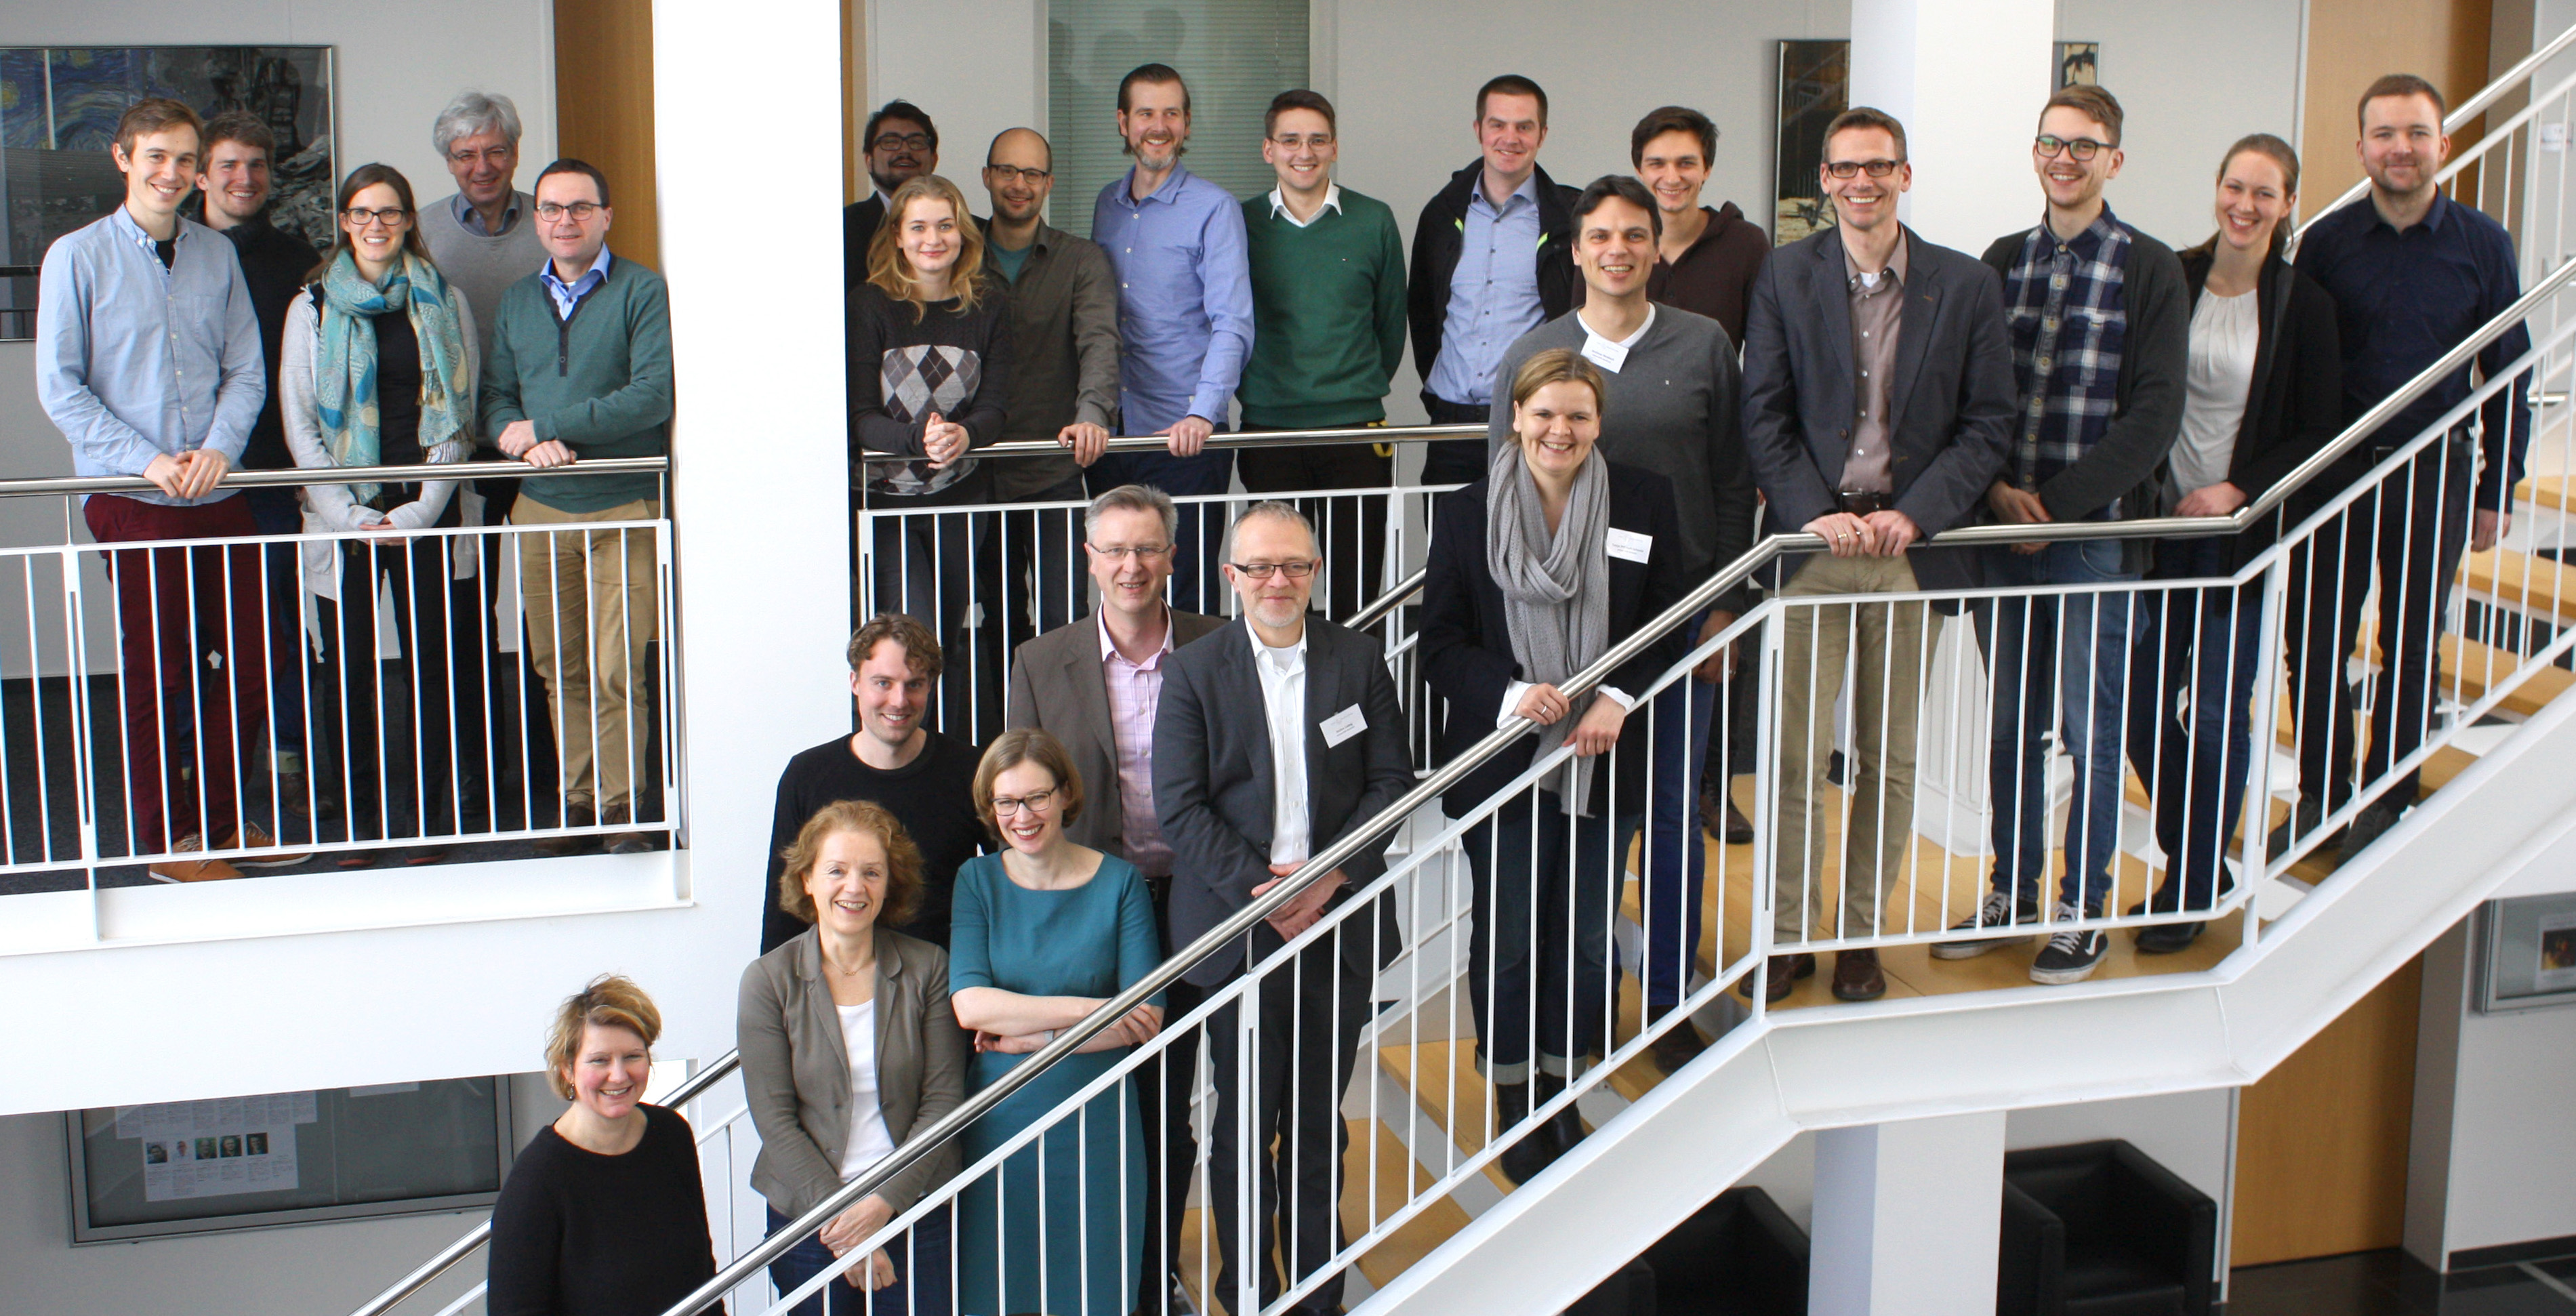
\includegraphics[width=0.8\linewidth]{figures/slides_for.jpg}}
\note{
   \begin{itemize}
      \item Hanse-Wissenschaftskolleg Delmenhorst 2017
   \end{itemize}
}
\end{frame}


%%%%%%%%%%%
% FOLIE 6 %
%%%%%%%%%%%
\begin{frame}{\vspace*{10mm}1\hspace*{1em}Vorgeschichte}
\frame{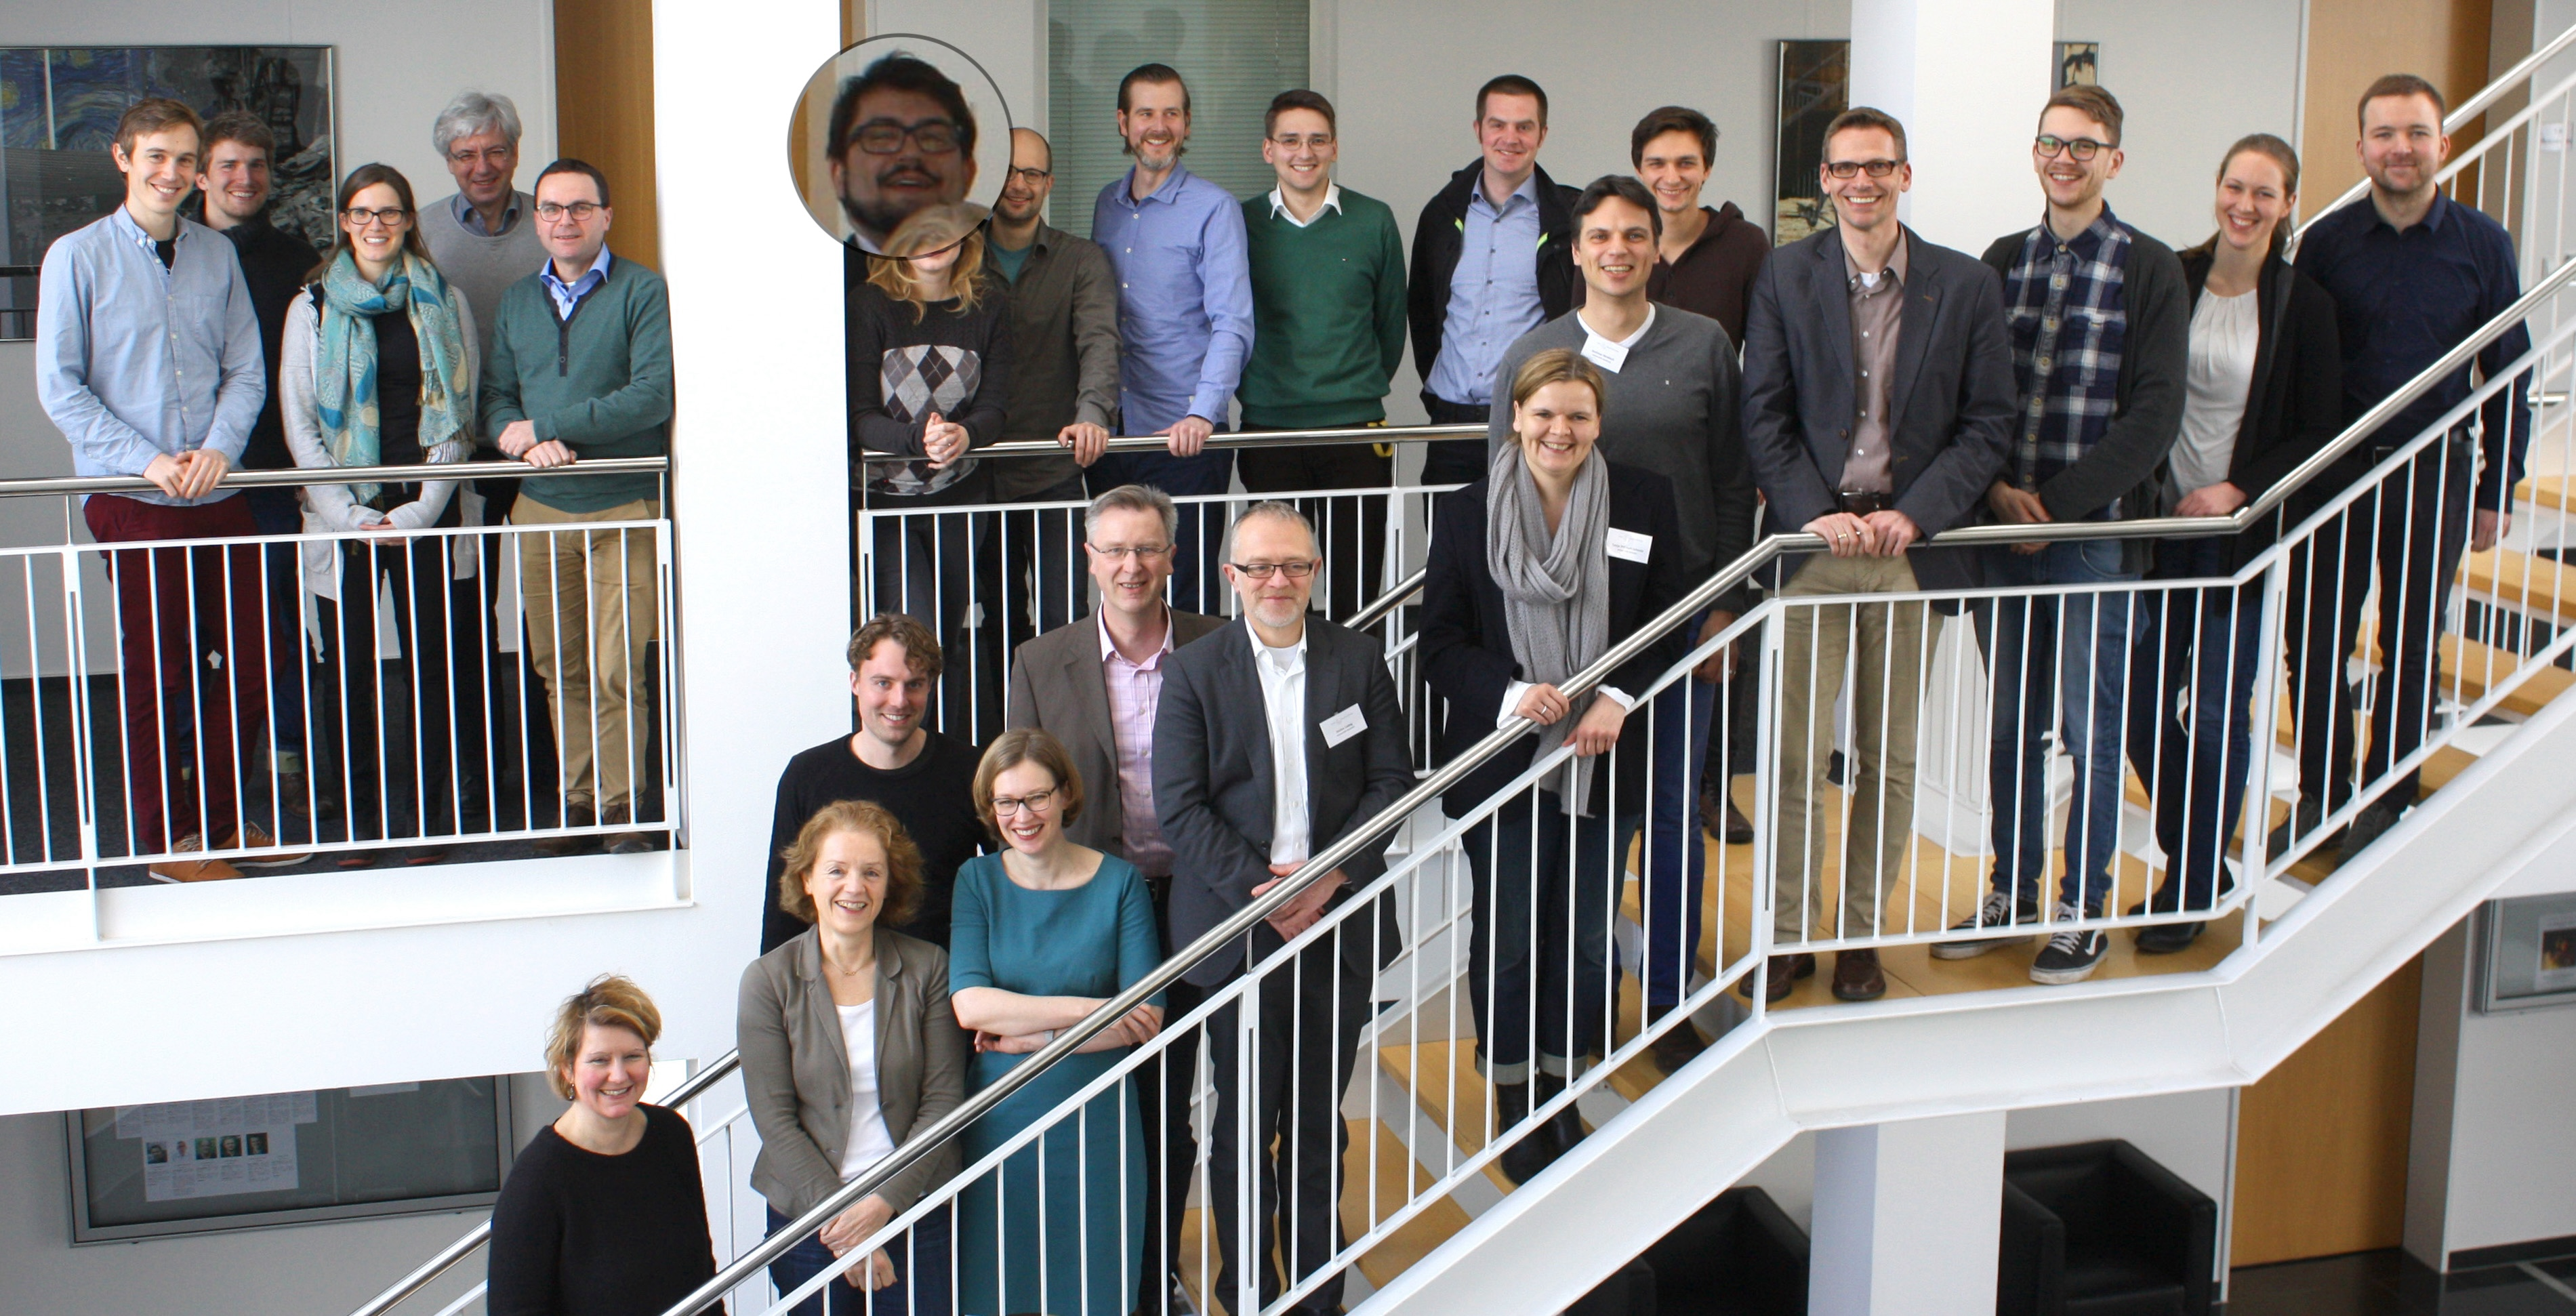
\includegraphics[width=0.8\linewidth]{figures/slides_for_close_up.jpg}}
\end{frame}


%%%%%%%%%%%
% FOLIE 7 %
%%%%%%%%%%%
\begin{frame}
\begin{overlayarea}{\textwidth}{0.81\paperheight}{
   \vspace*{11mm}
   \usebeamerfont{title}\textcolor{uolblue}
   {2\hspace*{1em}Empirische Forschung\\\hspace*{1.5em}und normative Theorie}
}
\vspace*{7mm}
\end{overlayarea}
\end{frame}


%%%%%%%%%%%
% FOLIE 8 %
%%%%%%%%%%%
\begin{frame}{\vspace*{10mm}2\hspace*{1em}Empirische Forschung und normative Theorie}
\begin{itemize}
   \item Deskriptive Ethik $\in$ Experimentelle Philosophie
   \item Experimentelle Philosophie $\in$ Philosophie
\end{itemize}
\end{frame}


%%%%%%%%%%%
% FOLIE 9 %
%%%%%%%%%%%
\begin{frame}{\vspace*{10mm}2\hspace*{1em}Empirische Forschung und normative Theorie}
\begin{multicols}{2}
\begin{itemize}
   \item \enquote{komplementäre Angewiesenheit [...] von empirischer Gerechtigkeitsforschung und normativer Gerechtigkeitstheorie} \textcolor{gray}{(Honneth 2008, S. 10)}
   \item Experimentelle Philosophie kann einen Beitrag zur Ethik leisten
   \begin{itemize}
      \item Erweiterung der Grundgesamtheit an Introspektionen, die zur Reflexion zur Verfügung stehen
      \item Falsifikation oder Verifikation empirischer Pr\"amissen
      \item Ex-ante- und Ex-post Evaluation der Implementation
   \end{itemize}
\end{itemize}
\vfill
\begin{center}
   \vspace{1cm}
   \frame{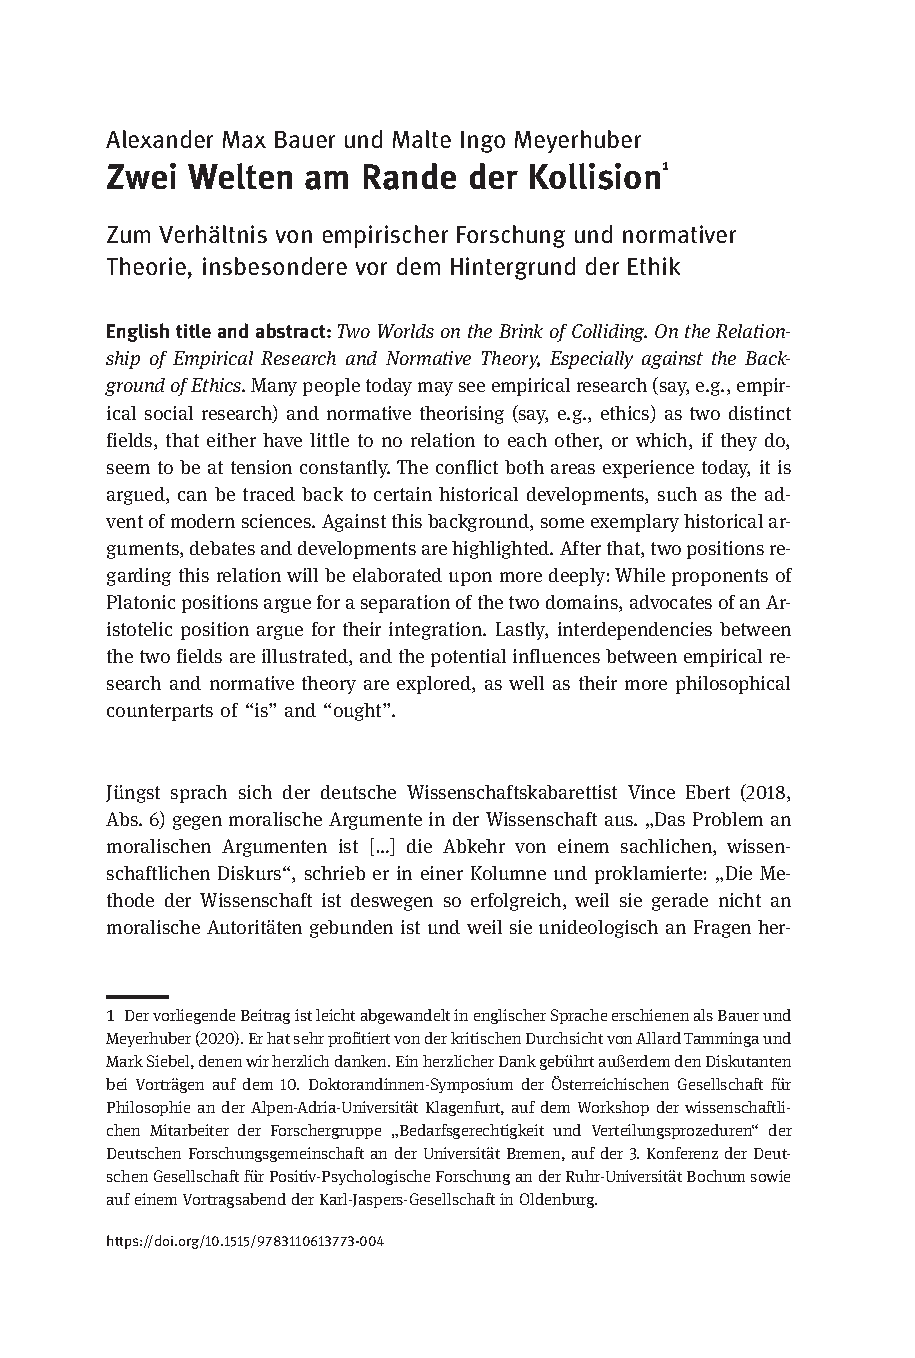
\includegraphics[width=0.6\linewidth]{figures/slides_bauer_meyerhuber_2019.pdf}}\\
   \footnotesize{\textcolor{gray}{Bauer und Meyerhuber 2019}}
   \vspace{1cm}
\end{center}
\end{multicols}
\note{
   \begin{itemize}
      \item kein naiver Positivismus
      \item \enquote{platonische} und \enquote{aristotelische} Perspektive \textcolor{gray}{(Miller 1994, S. 177ff.)}
   \end{itemize}
}
\end{frame}


%%%%%%%%%%%%
% FOLIE 10 %
%%%%%%%%%%%%
\begin{frame}
\begin{overlayarea}{\textwidth}{0.81\paperheight}{
   \vspace*{11mm}
   \usebeamerfont{title}\textcolor{uolblue}
   {3\hspace*{1em}Bedarf und Bedarfsgerechtigkeit}
}
\vspace*{7mm}
\end{overlayarea}
\end{frame}


%%%%%%%%%%%%
% FOLIE 11 %
%%%%%%%%%%%%
\begin{frame}{\vspace*{10mm}3\hspace*{1em}Bedarf und Bedarfsgerechtigkeit}
\begin{multicols}{2}
\begin{itemize}
   \item \enquote{So hat [...] Simonides nach Dichterart angedeutet, was das Gerechte sei: daß man jedem gebe, was ihm gebühre, und hat dies als Schuldigkeit bezeichnet} \textcolor{gray}{(Platon 2004, S. 13, 332\,b--c)}
   \item \enquote{Von der Gerechtigkeit im speziellen Sinn und dem in ihrem Sinne Gerechten findet sich die eine Form bei der Verteilung von Ehre, Geld oder anderen Gütern, die unter den Mitgliedern der Staatsgemeinschaft teilbar sind} \textcolor{gray}{(Aristoteles 2011, S. 166, 1130\,b)}
\end{itemize}
\vfill

\begin{center}
   \vspace{1cm}
   \frame{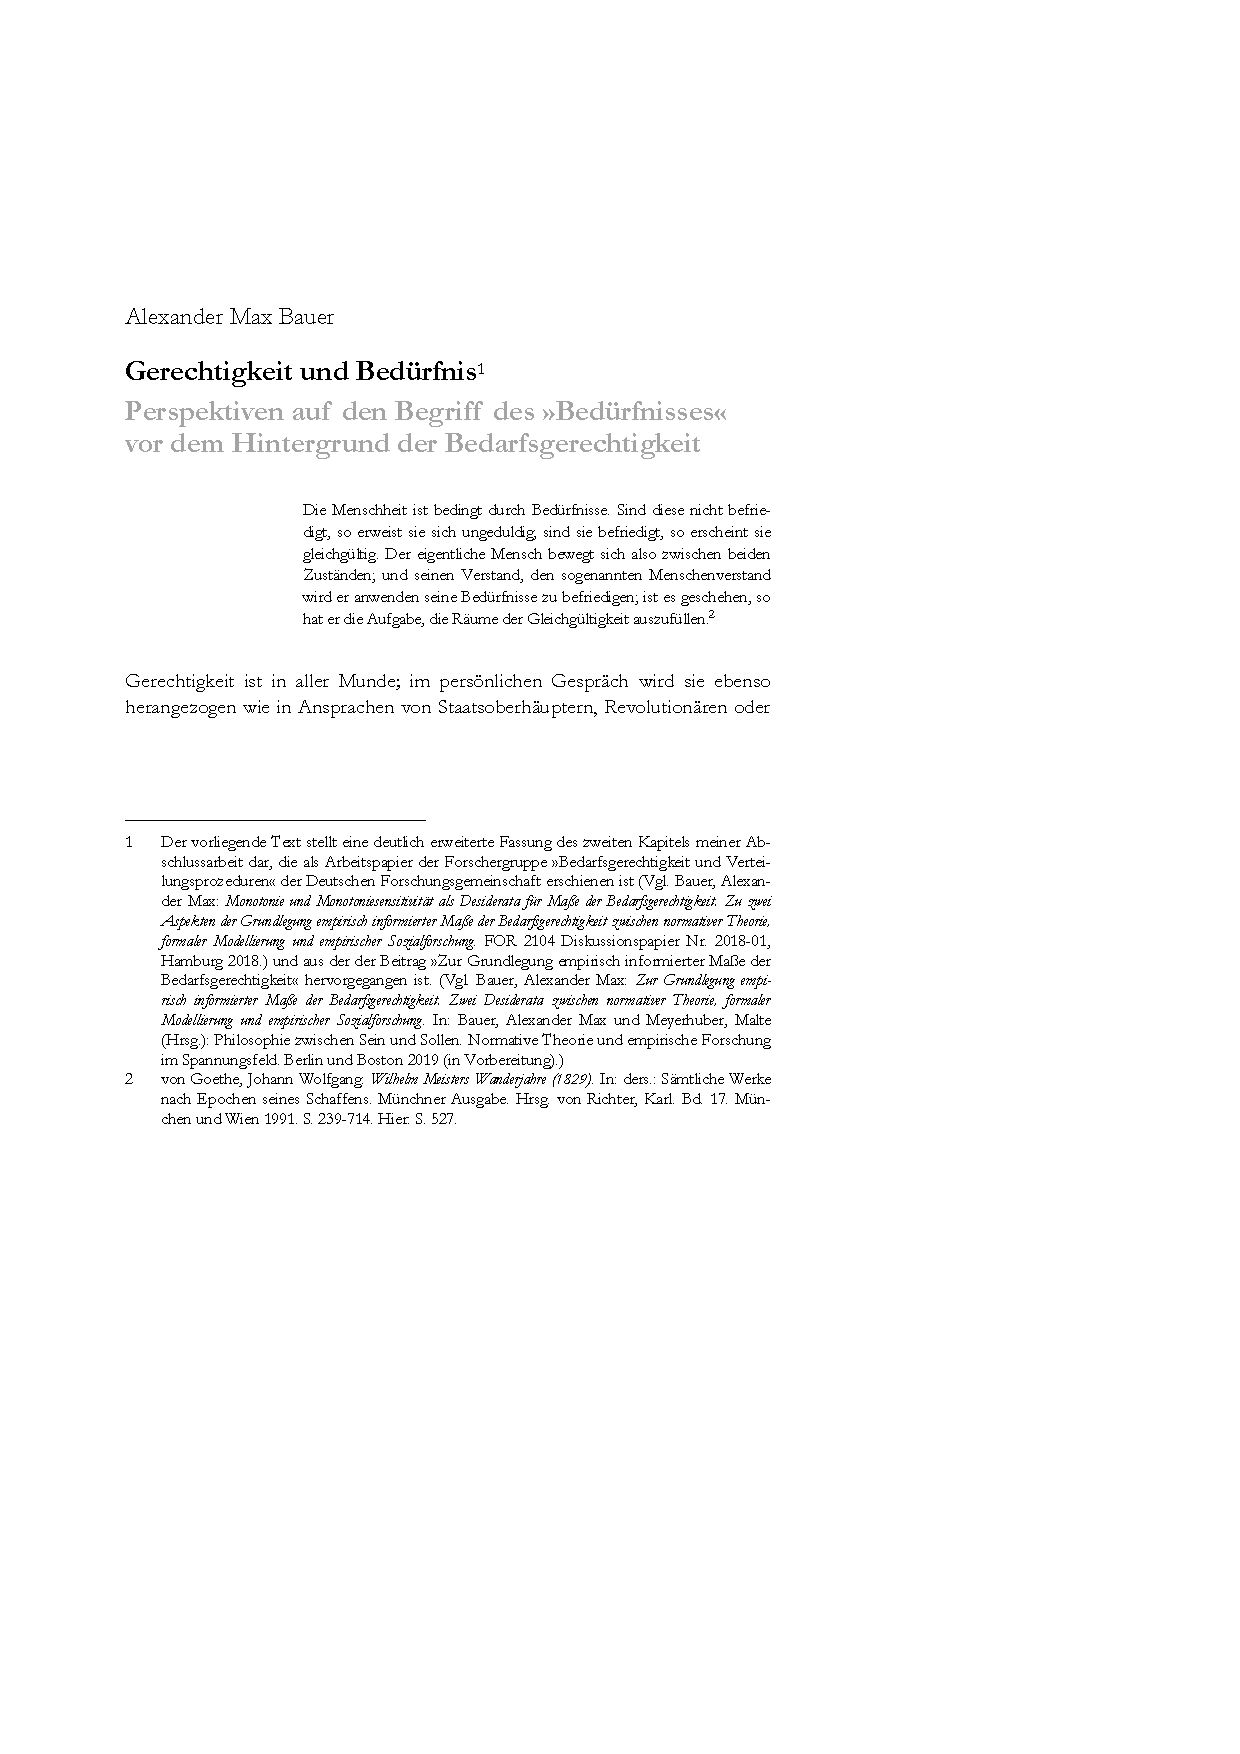
\includegraphics[width=0.6\linewidth]{figures/slides_bauer_2019.pdf}}\\
   \footnotesize{\textcolor{gray}{Bauer 2019}}
   \vspace{1cm}
\end{center}
\end{multicols}
\end{frame}


%%%%%%%%%%%%
% FOLIE 12 %
%%%%%%%%%%%%
\begin{frame}
\begin{overlayarea}{\textwidth}{0.81\paperheight}{
   \vspace*{11mm}
   \usebeamerfont{title}\textcolor{uolblue}
   {4\hspace*{1em}Bedarf als Referenzpunkt}
}
\vspace*{7mm}
\end{overlayarea}
\end{frame}


%%%%%%%%%%%%
% FOLIE 13 %
%%%%%%%%%%%%
\begin{frame}{\vspace*{10mm}4\hspace*{1em}Bedarf als Referenzpunkt}
\begin{multicols}{2}
\begin{itemize}
   \item Lorem
   \item Ipsum
   \item Dolor
\end{itemize}
\vfill

\begin{center}
   \vspace{1cm}
   \frame{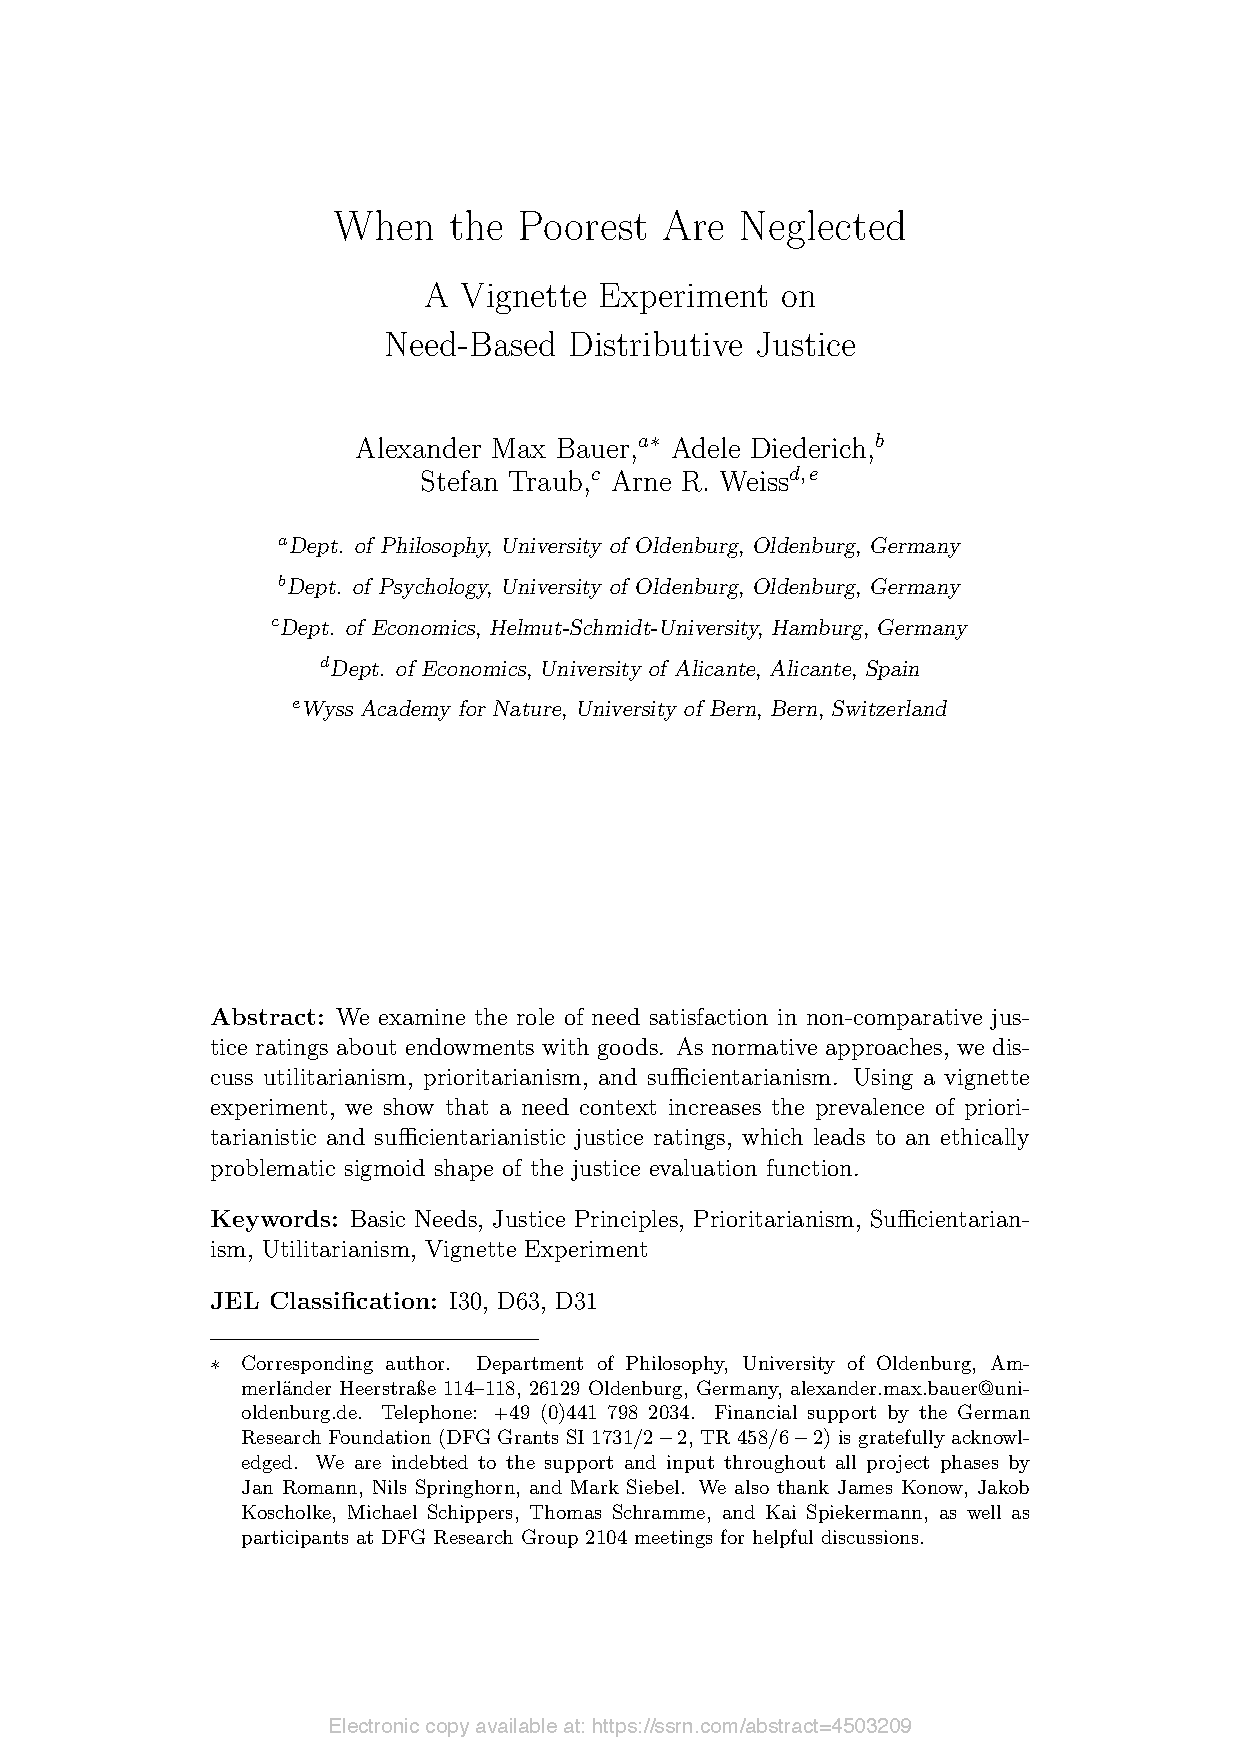
\includegraphics[width=0.6\linewidth]{figures/slides_bauer_et_al_2023a.pdf}}\\
   \footnotesize{\textcolor{gray}{Bauer et al. 2023a}}
   \vspace{1cm}
\end{center}
\end{multicols}
\end{frame}


%%%%%%%%%%%%
% FOLIE 14 %
%%%%%%%%%%%%
\begin{frame}
\begin{overlayarea}{\textwidth}{0.81\paperheight}{
   \vspace*{11mm}
   \usebeamerfont{title}\textcolor{uolblue}
   {5\hspace*{1em}Bedarf und Verantwortung}
}
\vspace*{7mm}
\end{overlayarea}
\end{frame}


%%%%%%%%%%%%
% FOLIE 15 %
%%%%%%%%%%%%
\begin{frame}{\vspace*{10mm}5\hspace*{1em}Bedarf und Verantwortung}
\begin{multicols}{2}
\begin{itemize}
   \item Lorem
   \item Ipsum
   \item Dolor
\end{itemize}
\vfill

\begin{center}
   \vspace{1cm}
   \frame{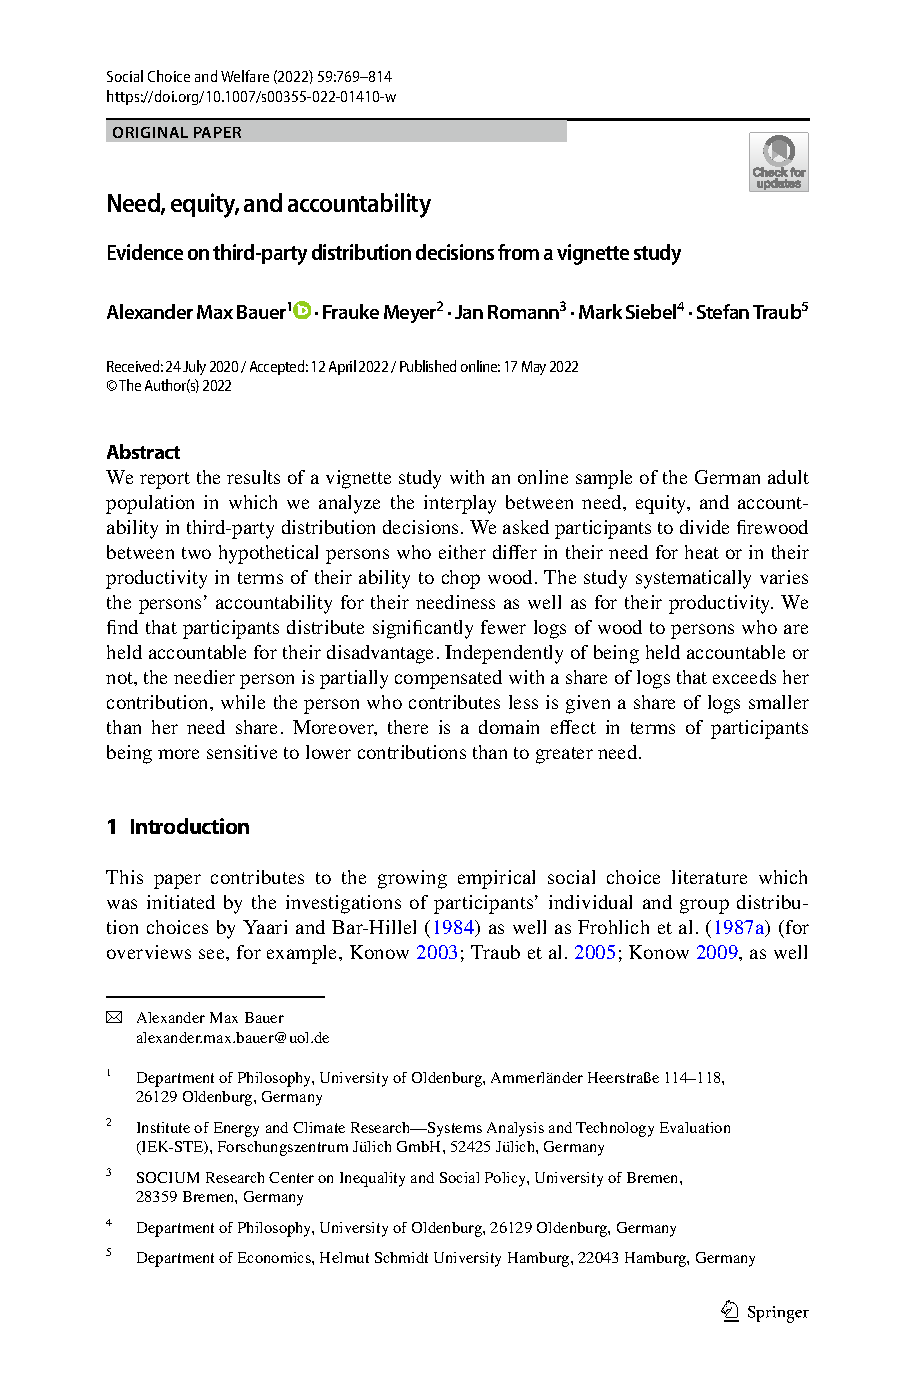
\includegraphics[width=0.6\linewidth]{figures/slides_bauer_et_al_2022.pdf}}\\
   \footnotesize{\textcolor{gray}{Bauer et al. 2022}}
   \vspace{1cm}
\end{center}
\end{multicols}
\end{frame}


%%%%%%%%%%%%
% FOLIE 16 %
%%%%%%%%%%%%
\begin{frame}
\begin{overlayarea}{\textwidth}{0.81\paperheight}{
   \vspace*{11mm}
   \usebeamerfont{title}\textcolor{uolblue}
   {6\hspace*{1em}Bedarfsarten}
}
\vspace*{7mm}
\end{overlayarea}
\end{frame}


%%%%%%%%%%%%
% FOLIE 17 %
%%%%%%%%%%%%
\begin{frame}{\vspace*{10mm}6\hspace*{1em}Bedarfsarten}
\begin{multicols}{2}
\begin{itemize}
   \item Lorem
   \item Ipsum
   \item Dolor
\end{itemize}
\vfill

\begin{center}
   \vspace{1cm}
   \frame{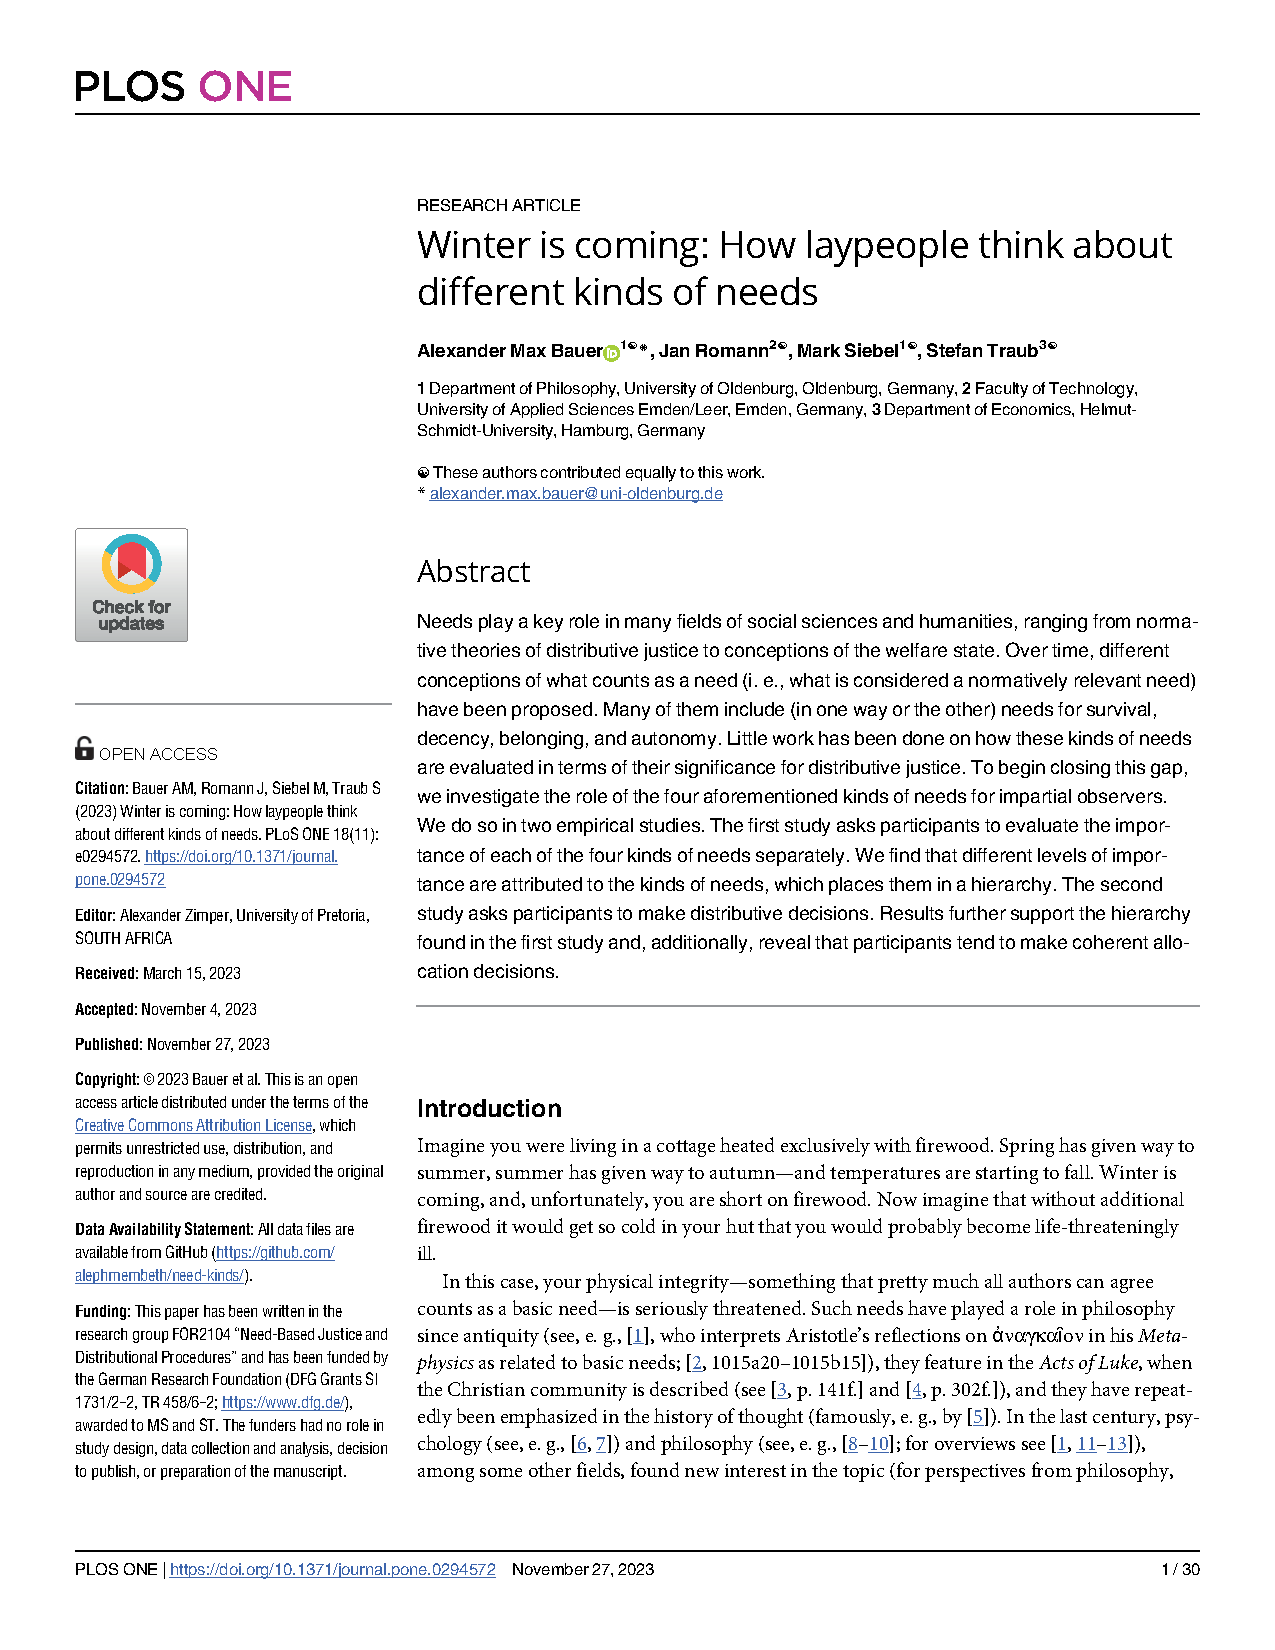
\includegraphics[width=0.6\linewidth]{figures/slides_bauer_et_al_2023b.pdf}}\\
   \footnotesize{\textcolor{gray}{Bauer et al. 2023b}}
   \vspace{1cm}
\end{center}
\end{multicols}
\end{frame}


%%%%%%%%%%%%
% FOLIE 18 %
%%%%%%%%%%%%
\begin{frame}
\begin{overlayarea}{\textwidth}{0.81\paperheight}{
   \vspace*{11mm}
   \usebeamerfont{title}\textcolor{uolblue}
   {7\hspace*{1em}Zusammenfassung\\\hspace*{1.5em}zentraler Ergebnisse}
}
\vspace*{7mm}
\end{overlayarea}
\end{frame}


%%%%%%%%%%%%
% FOLIE 19 %
%%%%%%%%%%%%
\begin{frame}{\vspace*{10mm}7\hspace*{1em}Zusammenfassung zentraler Ergebnisse}
\vspace*{-10mm}
\begin{itemize}
   \item[(1)] Unparteiische Beobachter*innen nehmen graduelle Gerechtigkeitseinschätzungen vor
   \item[(2)] Diese Einschätzungen sind abhängig von Versorgungssituationen
   \item[(3)] Bedarfsinformationen beeinflussen diese Einschätzungen
\end{itemize}

\vspace{1em}
\begin{itemize}
   \item[(4)] Unparteiische Entscheider*innen berücksichtigen Bedarf, Leistung und Verantwortung
   \item[(5)] Auch bei zu geringer Leistung wird Bedarf teilweise kompensiert
   \item[(6)] Kompensationsbereitschaft sinkt, wenn zu geringe Leistung selbst verschuldet ist
\end{itemize}

\vspace{1em}
\begin{itemize}
   \item[(7)] Unparteiische Beobachter*innen und Entscheider*innen unterscheiden Bedarfsarten
\end{itemize}
\end{frame}


%%%%%%%%%%%%
% FOLIE 20 %
%%%%%%%%%%%%
\begin{frame}{}

\includegraphics[width=0.8\linewidth]{figures/slides_thanks.pdf}
\end{frame}


%%%%%%%%%%%%
% FOLIE 21 %
%%%%%%%%%%%%
\begin{frame}{\vspace*{10mm}Bibliografie}
\vspace*{-4mm}
{\footnotesize
\begin{itemize}[label=,leftmargin=2em,itemindent=-2em]
   \item Bauer, Alexander Max (2019): \enquote{Gerechtigkeit und Bedürfnis. Perspektiven auf den Begriff des \enquote{Bedürfnisses} vor dem Hintergrund der Bedarfsgerechtigkeit}. In: Alexander Max Bauer und Nils Baratella (Hrsg.): \textit{Oldenburger Jahrbuch für Philosophie 2017/2018}. Oldenburg: BIS-Verlag. S. 285--327.
   \item Bauer, Alexander Max, Adele Diederich, Stefan Traub und Arne Robert Weiss (2023): \enquote{When the Poorest Are Neglected. A Vignette Experiment on Need-Based Distributive Justice}. \textit{SSRN Working Paper} 4503209.
   \item Bauer, Alexander Max, Frauke Meyer, Jan Romann, Mark Siebel und Stefan Traub (2022): \enquote{Need, Equity, and Accountability. Evidence on Third-Party Distributive Decisions from a Vignette Study}. In: \textit{Social Choice and Welfare} 59, S. 769--814.
   \item Bauer, Alexander Max und Malte Ingo Meyerhuber (2019): \enquote{Zwei Welten am Rande der Kollision. Zum Verhältnis von empirischer Forschung und normativer Theorie, insbesondere vor dem Hintergrund der Ethik}. In: dies. (Hrsg.): \textit{Philosophie zwischen Sein und Sollen. Normative Theorie und empirische Forschung im Spannungsfeld}. Berlin und Boston: Walter de Gruyter. S. 13--37.
   \item Bauer, Alexander Max und Jan Romann (i.\,V.): \enquote{Equal Deeds, Different Needs. Need, Accountability, and Ressource Availability in Third-Party Distributive Decisions}. In: Shaun Nichols und Joshua Knobe (Hrsg.): \textit{Oxford Studies in Experimental Philosophy}. Oxford: Oxford University Press.
   \item Bauer, Alexander Max, Jan Romann, Mark Siebel und Stefan Traub (2023): \textit{Winter is Coming. How Laypeople Think About Different Kinds of Needs}. \textit{PLOS ONE}
   \item Bauer, Alexander Max und Mark Siebel (i.\,V.): \enquote{Measuring Need-Based Distributive Justice -- Formally and Empirically}. In: Stefan Traub und Bernhard Kittel (Hrsg.): \textit{Priority of Needs. An Informed Theory of Need-Based Justice}. Cham: Springer.
\end{itemize}
}
\end{frame}


%%%%%%%%%%%%
% FOLIE 22 %
%%%%%%%%%%%%
\begin{frame}
\begin{overlayarea}{\textwidth}{0.81\paperheight}
   {
   \vspace*{11mm}
   \usebeamerfont{title}\textcolor{uolblue}
   {Zusätzliche Folien}
   }
\end{overlayarea}
\end{frame}


%%%%%%%%%%%%
% FOLIE 23 %
%%%%%%%%%%%%
\begin{frame}{\vspace*{10mm}2\hspace*{1em}Empirische Forschung und normative Theorie}
\frame{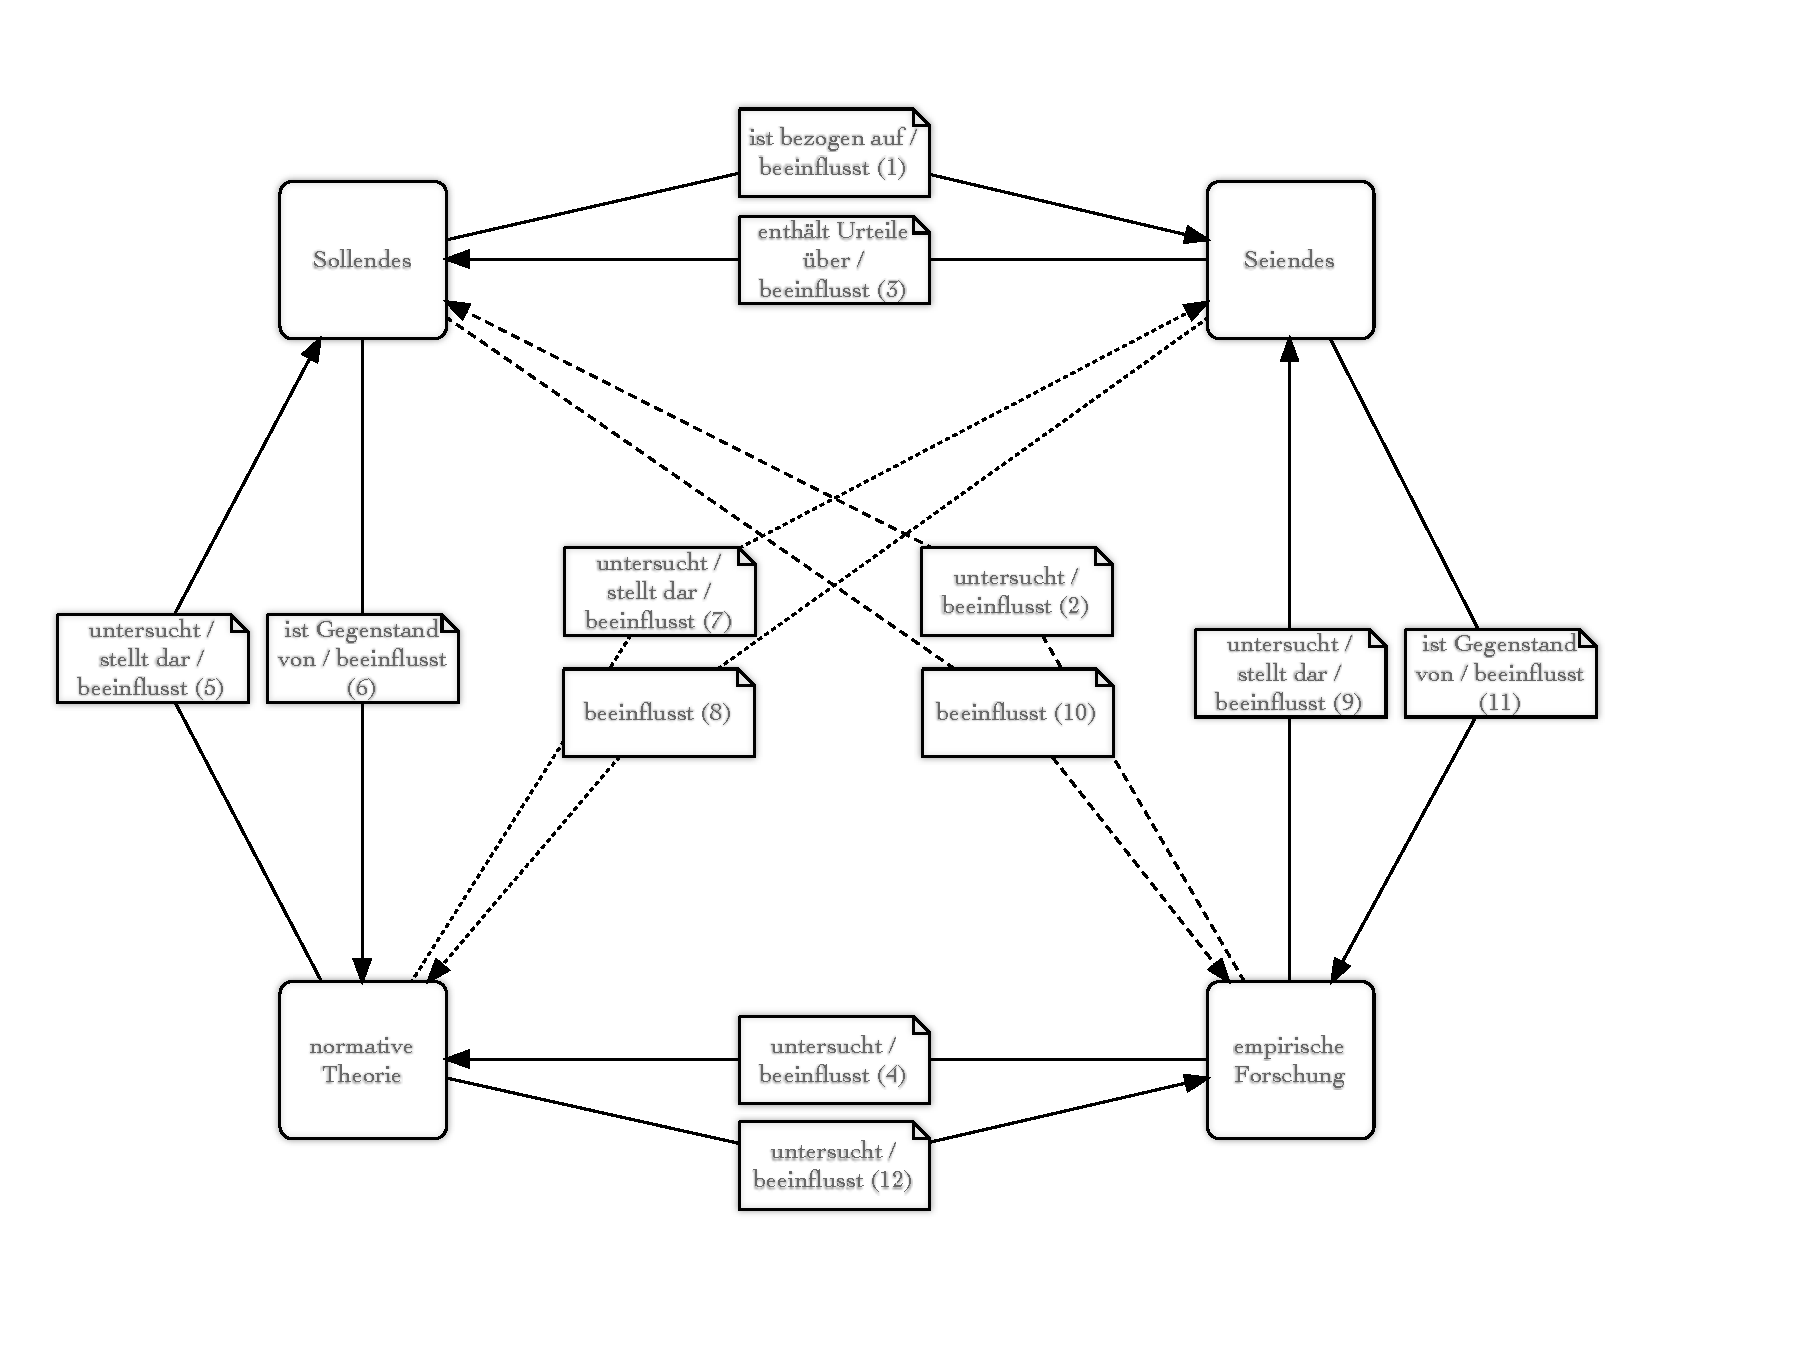
\includegraphics[width=0.6\linewidth]{figures/slides_emp_norm.pdf}}\\
\footnotesize{\textcolor{gray}{Bauer und Meyerhuber 2019, S. 26}}
\end{frame}

\end{document}
